\section{Gameplay y Mecánicas}
\subsection{Gameplay}
\subsubsection{Progresión del juego}
Run or Wake tiene como mecánica principal el esquivar obstáculos
mientras el personaje corre y aumenta la velocidad del juego a medida
que pasa el tiempo. Además de la recolección de almuadas hasta alcanzar
la cuota establecida en cada nivel para desbloquear el siguiente.
\subsubsection{Misión / estructura del los desafíos}
Se basa en que el personaje (protagonista/jugador) pueda recolectar una 
cantidad de almuadas mostradas en la interfaz y cumplir con la cuota en cada nivel, mientras
esquivan obstáculos, escapando de un monstruo (antagonista / Enemigo).

\begin{table}[!ht]
  \begin{center}
    \begin{tabular}{| c | c |}
      \hline
      Nivel & Cantidad de almuadas \\ \hline
      Nivel 1 & 30 estrellas \\ \hline
      Nivel 2 & 40 estrellas \\ \hline
      Nivel 3 & 60 estrellas \\ \hline
    \end{tabular}
    \caption{Cantidad de almuadas recolectadas como misión}
    \label{tab:estrellas}
  \end{center}
\end{table}

\subsubsection{ Objetivos - ¿Cuáles son los objetivos del juego ?}
Run or Wake tiene como objetivo el escapar de su pesadilla, recolectar
la cantidad de estrellas mencionadas en la tabla \ref{tab:estrellas}
y por supuesto alcanzar la mejor puntuación. Aportando así a la obtención
de un espíritu competitivo.

\subsubsection{ Play flow - ¿ Cómo es la experiencia del juego para el jugador ?}

El juego ofrece al jugador la posibilidad de mejorar sus reflejos, la posibilidad
de entretenerse y obtener un momento de demostrar sus habilidades motrices y de 
coordinación motora entre su sentido de la vista y sus dedos.\\

En general, la experiencia del jugador con Run or Wake resulta muy gratificante, ya 
ofrece desafíos retadores en cada nivel del juego además de unos escenarios hermosos
que serán gratos de observar.

\subsection{Mecánicas}
¿Cuáles serán las reglas del juego?, ambas implícitas y explicitas. Este es el modelo del 
universo con el cual el juego trabaja. Es como una simulación del mundo. ¿De qué forma interactuan
todas las piezas? Este es uno de los apartados más largos e importantes del GDD.

\subsubsection{Físicas - ¿Cómo funciona la física?}

La física del juego es igual al mundo real con un aproximado de $9.8 m/s^2 $

\subsubsection{Movimiento}
\begin{itemize}
  \item \textbf{Movimiento general}: El movimiento general es hacia adelante automático (running)
  \item \textbf{Otros tipos de movimientos}: Los movimientos del personaje son
    hacia la izquierda, hacia la derecha y  saltar.
\end{itemize}

\subsubsection{Objetos}
\begin{itemize}
  \item \textbf{Obtener objetos}: Puntos
  \item \textbf{Mover objetos}: NO
\end{itemize}

\subsubsection{Acciones}
\begin{itemize}
  \item \textbf{Botones y palancas}:  teclas flechas.
\end{itemize}

\subsubsection{Economía- ¿Cuál es la economía del juego? ¿Cómo funciona esta?}
La economía funciona mediante la recolección de almuadas que se encuentran en el
camino.

\subsection{ Flujo de pantallas}

\begin{figure}[!ht]
  \centering
  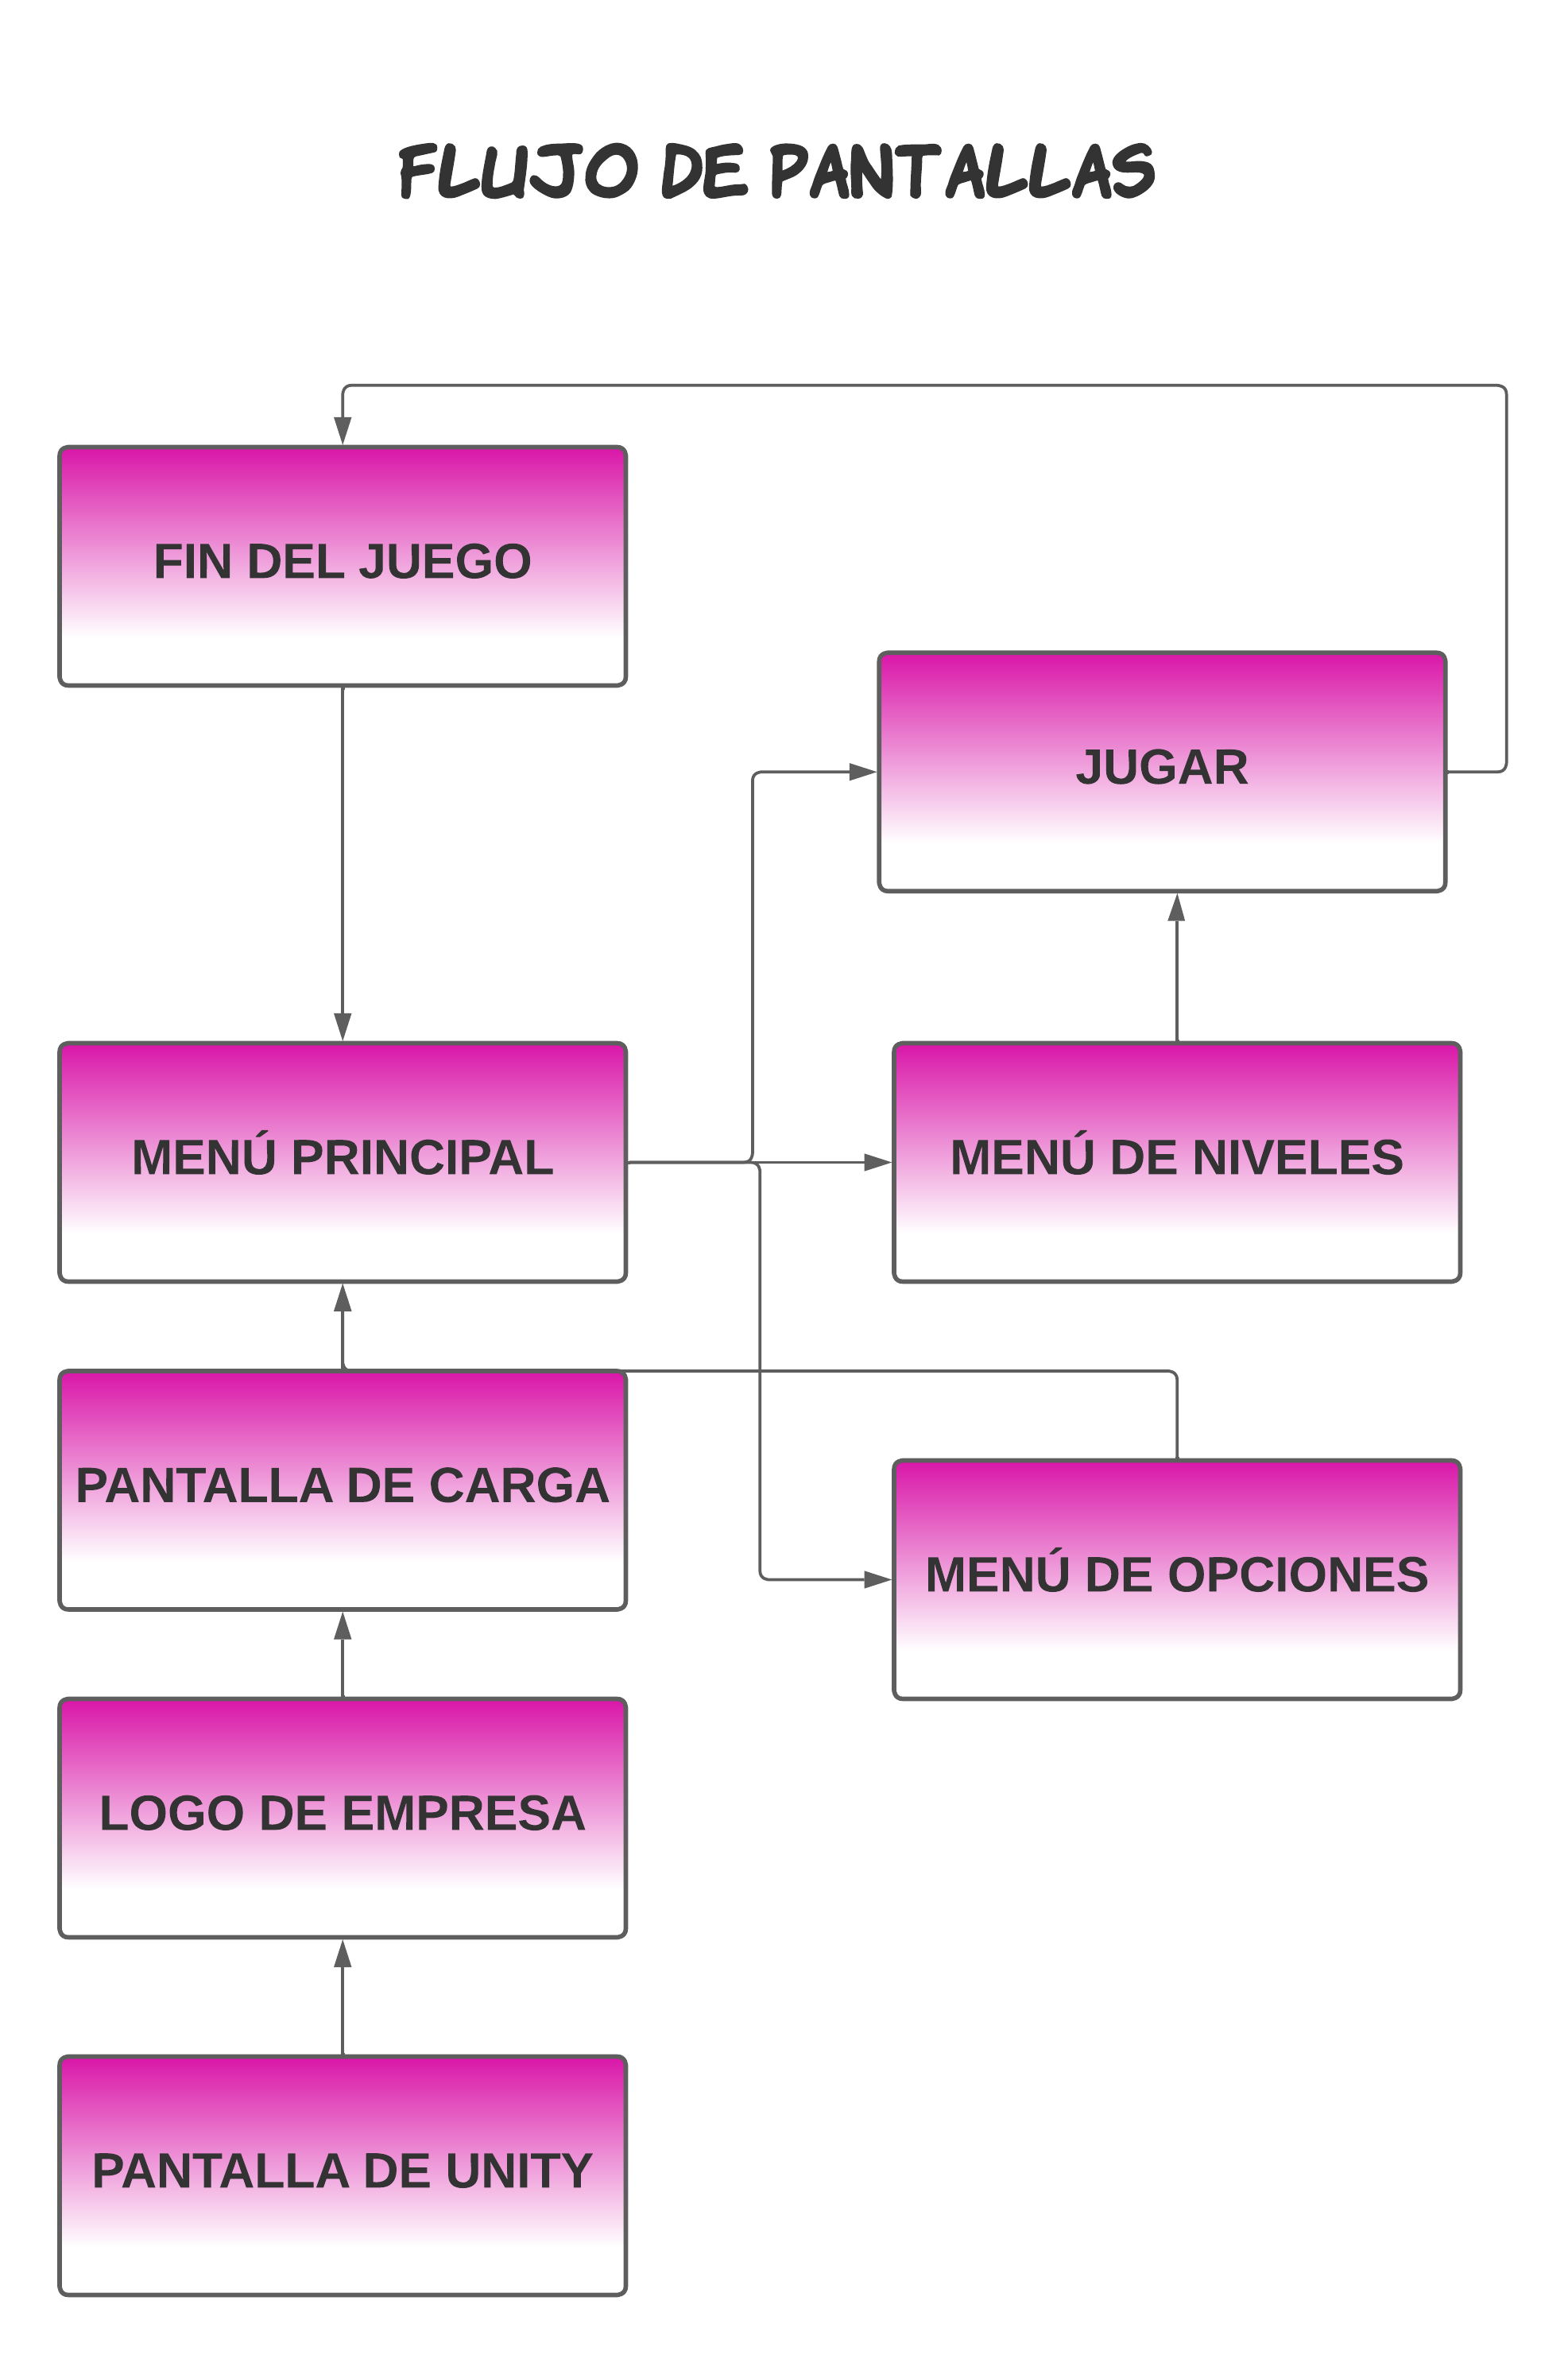
\includegraphics[scale = 0.7]{Figures/0. General/pantallas.png}
  \caption{Caption goes here}
  \label{fig:myfigure}
\end{figure}

\subsubsection{Descripción de pantallas - ¿Cuál es el propósito de cada pantala}
\begin{itemize}
  \item \textbf{Pantalla del menú del juego}
    \begin{itemize}
      \item \textbf{Jugar}: Esta acción te llevará al escenario del juego
      \item \textbf{Opciones}: Esto te llevará al menú de opciones donde tendrás
        la posibilidad de ajustar el brillo y volumen del juego.
      \item \textbf{Salir}: Con este botón sales del juego
    \end{itemize}
  \item \textbf{Pantalla de Opciones}
    \begin{itemize}
      \item \textbf{Volumen}: Para poder ajustar el volumen del juego
      \item \textbf{Intensidad de brillo}: Para ajustar el brillo
    \end{itemize}
\end{itemize}


